\section{Evaluation}
\subsection{Datasets}
 Both real-world and synthetic datasets were used to evaluate and compare the approximate Monte Carlo method to the standard PageRank method. The real-world datasets were obtained from the Stanford Network Analysis Project (SNAP), a well-known repository of large graph datasets \cite{standford_university_snap_2025}. It includes social networks, web graphs, and communication networks, among others. These datasets such as wiki-Talk are publicly available and can be downloaded from the SNAP website. These graphs have realistic structures with millions of nodes and edges. \par
Furthermore, synthetic graphs of any size and with different characteristics can be generated. In the experiments, Erdős–Rényi graphs of different sizes, ranging from $100.000$ to $20$ million nodes, have been generated. To establish comparable conditions between the different graph sizes, the density is kept consistent by controlling the number of outgoing edges per node. However, the in-degree of each node is random and ranges between $0$ and $n-1$, where $n$ is the total number of nodes. A simple python script was used to generate and store the graph structure in an edge list file.

\vspace{1.0em}
\begin{algorithm}[H]
\caption{Synthetic Graph Generator}
\KwIn{Range of node counts $[N_{\min}, N_{\max}]$, step size $\Delta N$, edges per node $E$}
\KwOut{Synthetic graph files with $E$ outgoing edges per node}

Set random seed for reproducibility\;
\For{$n \gets N_{\min}$ \KwTo $N_{\max}$ \KwStep $\Delta N$}{
  Create output file for graph with $n$ nodes\;
  \ForEach{node $u \in \{1, \dots, n\}$}{
    \For{$i \gets 1$ \KwTo $E$}{
      Select random destination $v \in \{1, \dots, n\}$\;
      \If{$v \neq u$}{
        Write edge $(u, v)$ to file\;
      }
    }
  }
  
}
\end{algorithm} 
\vspace{1.0em}

The selected datasets from SNAP vary in size, structure and density. The following table presents the chosen graphs and their characteristics: 

% include table
\begin{table}[ht]
\centering
\setlength{\tabcolsep}{6pt}
\renewcommand{\arraystretch}{1.2}
\begin{tabularx}{\linewidth}{l r r l X}
\toprule
\textbf{Dataset} & \textbf{Nodes} & \textbf{Edges} & \textbf{Type} & \textbf{Expected Behavior} \\
\midrule
wiki-Talk    & 2.4M & 5M    & Communication & Medium convergence \\
web-Google   & 875K & 5.1M  & Web Graph & Fast convergence, extreme authority \\
soc-Pokec    & 1.6M & 30.6M & Social Network & Slow convergence, distributed authority \\
web-BerkStan & 685K & 7.6M  & Web Graph & Fast convergence, dense connections \\
\bottomrule
\end{tabularx}
\caption{Benchmark datasets and expected behavior.}
\label{tab:datasets}
\end{table}



 %The real-world datasets selected from SNAP vary in size, density, and structure. Among them are:

%Wiki-Talk: A communication network from Wikipedia where a directed edge from user u to user v indicates that u has edited v’s talk page. This dataset contains millions of edges and is highly irregular, with some users having extremely high degree. It is one of the largest and most challenging graphs used in the experiments.

% Wiki-Vote: A voting network of Wikipedia users where edges represent votes cast in administrator elections. The dataset is smaller but directed, providing a good comparison for medium-sized graphs.

% Slashdot: A social network where edges represent “friend” or “foe” relationships between users. This dataset is useful because it represents a signed social graph with complex structure.

% Amazon Co-Purchasing Network: A product co-purchasing network where nodes are products and edges indicate that two products are often bought together. This dataset models a recommendation-style graph and offers a different type of degree distribution.


%\subsubsection{Data Sources of real-world Graphs}
% Description of synthetic and real-world datasets used


\subsection{Implementation in Spark}
% \subsubsection{Graph Representation with RDDs}
% \subsubsection{Adjacency List Construction}
% \subsubsection{Broadcasting for Teleportation}
% \subsubsection{Walker State Representation and Distribution}
% \subsubsection{RDD Caching, Materialization, and Unpersisting}
% \subsubsection{Repartitioning for Load Balancing}

The Monte Carlo Implementation is structured around two main components: The graph representation and the walker states. Both of them are stored in Sparks RDDs, which make them suitable for processing in a distributed system.\par

At the beginning of the program an edge list file is read to get the structure of the graph. It is stored as an RDD of directed edges. Then by grouping the outgoing neighbors of each node an adjacency list is constructed, which is one of the main RDD-based components, that is represnting the entire graph structure:

\vspace{0.5em}
\begin{lstlisting}[language=Scala, caption={Adjacency list creation}, label={lst:adjlist}]
val adjList: RDD[(Long, Iterable[Long])] = edgesRDD.groupByKey().cache()
\end{lstlisting}
\vspace{0.5em}

Additionally, an array of all vertices is required to support teleportation. This list will be distributed as a broadcasting variable to all nodes.

\vspace{0.5em}
\begin{lstlisting}[language=Scala, caption={Broadcasting Variable}, label={lst:broadcast}]
val broadcastNodes = sc.broadcast(allNodesArray)
\end{lstlisting}
\vspace{0.5em}

This mitigates costly network shuffles during every teleportation. Because the set of nodes is required in every simulation step it is cached in memory for efficient access.
A fixed number of walkers are initialized and represented in a seperate RDD. The RDD is distributed across multiple partitions to ensure efficient parallel processing and scaling when analyzing large graphs. Each entry in the RDD is a random vertex ID, representing the current vertex of a walker. In each simulation step the walker RDD is joined with the adjacency list to get all possible outgoing edges. After each walker updates its position, a new walker RDD is initialized with the updated positions. Before the previous walker RDD is explicitly unpersisted after the step is completed, the new walker RDD has to be materialized.
%\newpage
\begin{lstlisting}[language=Scala, caption={Materializing and Unpersisting Walker RDD}, label={lst:materialize}]
nextWalkersRDD.cache() 
nextWalkersRDD.count() // trigger an action to materialze RDD
walkersRDD.unpersist(blocking = false)
\end{lstlisting}
\vspace{0.5em}
This is because Spark uses lazy evaluation. It ensures that only the current walker RDD and the adjacency list occupy memory. \par
Before caching the walkers RDD in memory, repartitioning is applied to the RDD after each step. This is crucial for balanced distribution across partitions as it ensures that the number of partitions remains the same throughout the experiment. 
When processing large graphs that include nodes with high ingoing edges it prevents skews and stragglers allowing Spark to efficiently use all available cores. Managing the partitions correctly can have a significant impact on performance. 


\subsection{Experimental Framework and Automation}

% \subsubsection{Datasets: Real-World and Synthetic Graphs}
% \subsubsection{Synthetic Graph Generation}
% \subsubsection{Parameter Variation in Experiments}
% \subsubsection{Spark Cluster Setup}
% \subsubsection{Automation via Shell Scripts}
% \subsubsection{Data Collection and Visualization}

To evaluate the performance of the approximate Monte Carlo method an experimental framework was established, that aims for reproducibility. It benchmarks the Monte Carlo method and compares it to the standard PageRank method. The evaluation is focusing mainly on memory efficiency while trading off performance and accuracy. \par
% The datasets used for evaluation include both real-world and synthetic graphs. Real-world graphs such as wiki-Talk provide an irregular graph structure and millions of edges, presenting a practical use case. On the other hand, synthetic graphs of any size and with different characteristics can be generated. In the experiments, Erdős–Rényi graphs of different sizes, ranging from $100.000$ to $20$ million nodes, have been generated. To establish comparable conditions between the different graph sizes, the density is kept consistent by controlling the number of outgoing edges per node. However, the in-degree of each node is random and ranges between $0$ and $n-1$, where $n$ is the total number of nodes. A simple python script is used to generate and store the graph structure in an edge list file.

% \vspace{1.5em}
% \begin{algorithm}[H]
% \caption{Synthetic Graph Generator}
% \KwIn{Range of node counts $[N_{\min}, N_{\max}]$, step size $\Delta N$, edges per node $E$}
% \KwOut{Synthetic graph files with $E$ outgoing edges per node}

% Set random seed for reproducibility\;
% \For{$n \gets N_{\min}$ \KwTo $N_{\max}$ \KwStep $\Delta N$}{
%   Create output file for graph with $n$ nodes\;
%   \ForEach{node $u \in \{1, \dots, n\}$}{
%     \For{$i \gets 1$ \KwTo $E$}{
%       Select random destination $v \in \{1, \dots, n\}$\;
%       \If{$v \neq u$}{
%         Write edge $(u, v)$ to file\;
%       }
%     }
%   }
  
% }
% \end{algorithm} 
% \vspace{1.5em}

\par
During the experiments, the main parameters of the Monte Carlo method have been varied. The parameters include the number of walkers and the number of steps per walker. The goal was to systematically compare performance, memory and runtime across varying parameters. In the GraphX implementation the only parameters that were configured are the tolerance and the damping factor. The tolerance is usually set to $0.001$. In the experiments it was kept on such a low value to get very precise PageRank values and to compare the approximate Monte Carlo approach to the standard PageRank method. The reset probability was set to $0.15$ for both methods. Additionally, different Spark configurations were analyzed such as the number of executors and most importantly the memory allocated per executor. \par



To automate the experiments, shell scripts are used. Each script relies on spark-submit, which is the standard command line tool used to launch applications on a Spark cluster. In the spark-submit command configurations such as the number of executors and the memory per executor can be set. Furthermore, the edge list file is passed to the script as well as the Monte Carlo specific configuration such as the number of walkers and steps per walker. This setup ensures that experiments are running in a sequence without needing manual input and with consistency throughout multiple data sets. Finally, the spark-submit command allows to either run the applications locally or to launch them to a cluster environment to simulate a real distributed system. \par

\begin{figure}[H]
    \centering
    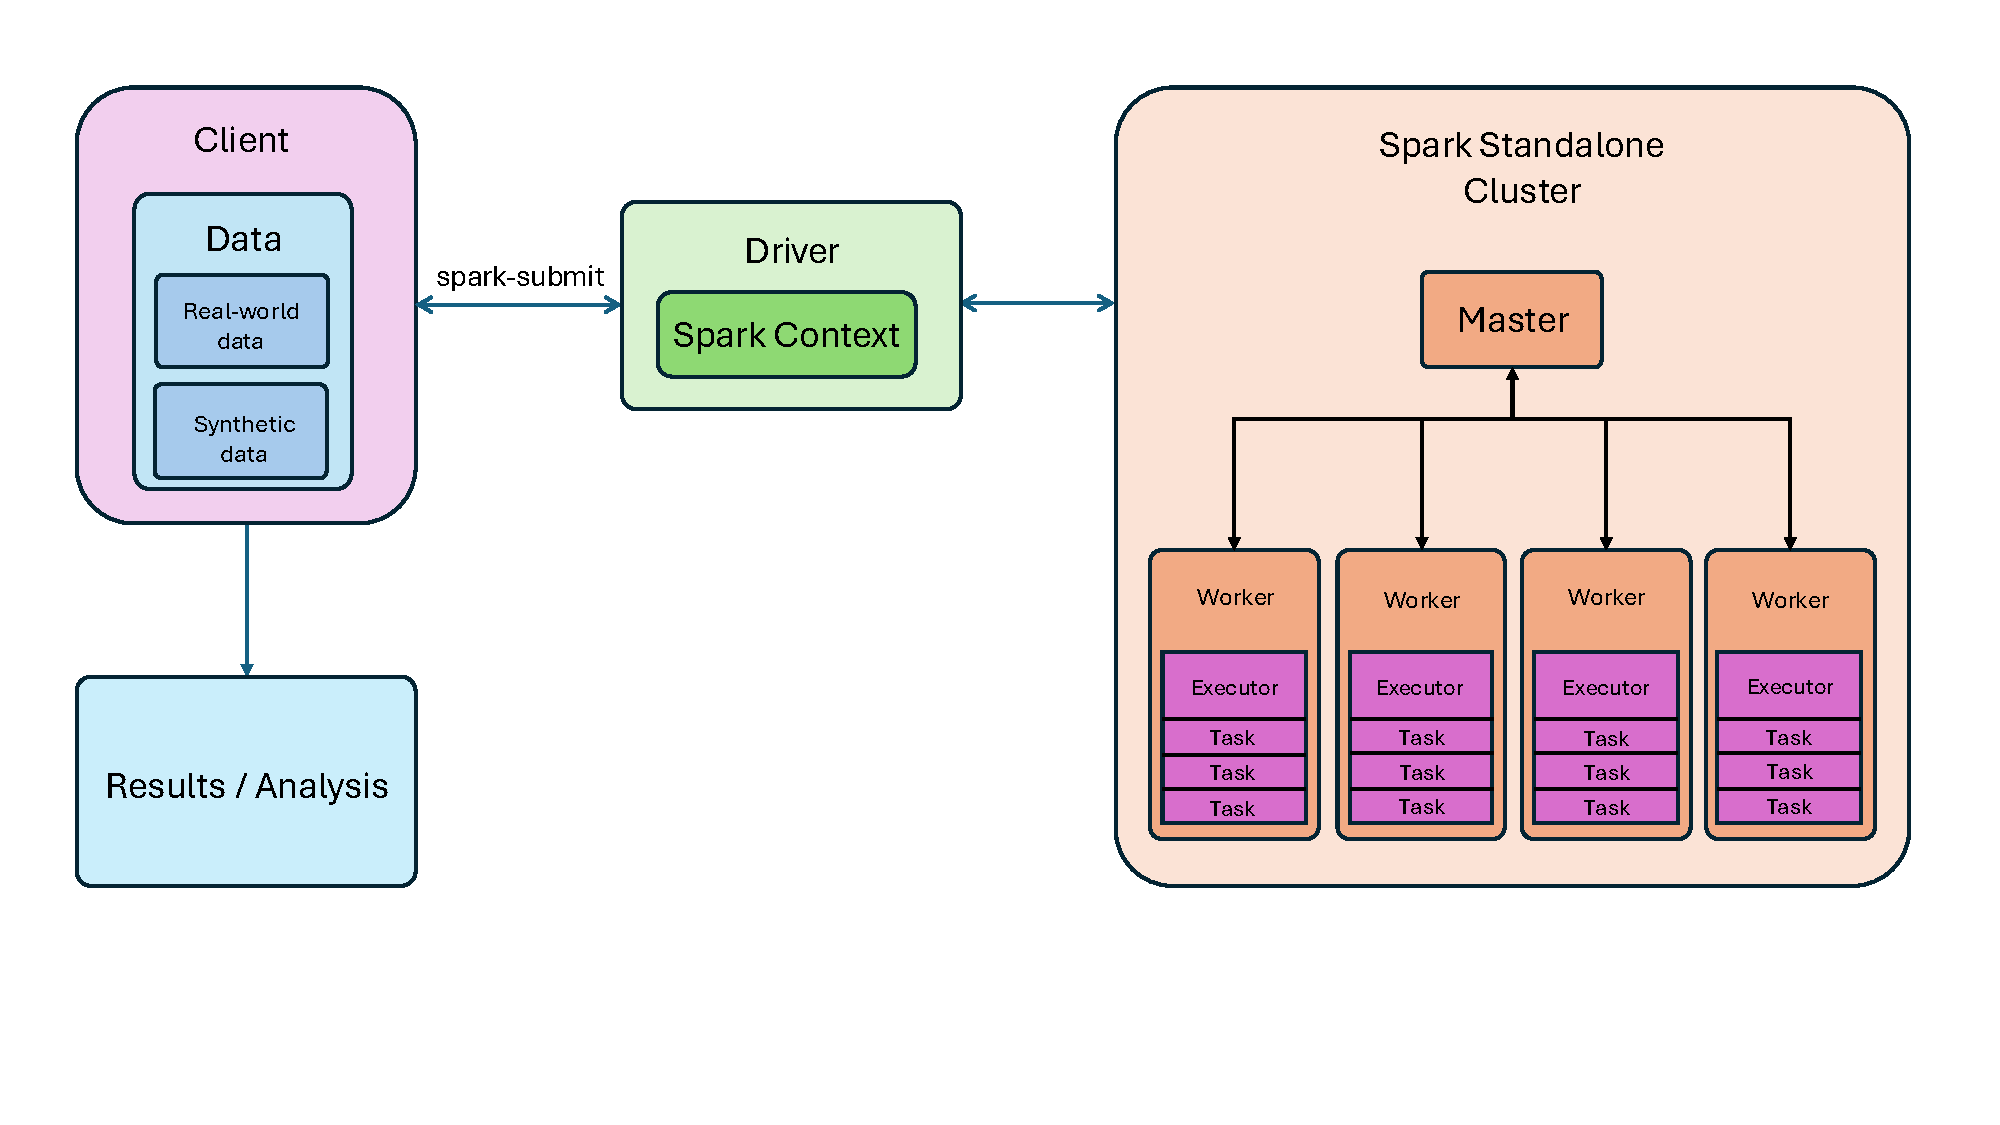
\includegraphics[width=\linewidth]{images/Workflow_image.pdf}
    \caption{Experimental Workflow}
    \label{fig:workflow}
\end{figure}
To ensure comparable conditions across all experiments, all experiments were executed on a Spark cluster set up on the university's server. For simplicity, the Spark cluster was deployed in standalone mode, which is a built-in cluster manager. Only the master and workers need to be started on the university server. The cluster consists of one master node and four worker nodes. Each worker node has one executor with two cores, for a total of eight cores. \par


In every experiment, metrics for both methods were collected, including configurations such as the number of walkers and steps for the Monte Carlo method. Another file collected the total runtime, allocated memory, and graph size to evaluate performance with limited memory and with different graph sizes. For accuracy evaluation, the top 20 ranks for both methods were saved in a separate file. \par
All the collected data was saved in CSV files to efficiently analyze it in the next step. With the help of Python scripts and the use of libraries such as Matplotlib and Pandas, the data is structured and visualized in various plots of runtime, allocated memory, accuracy and cost. This provides a clear overview of the data and enables a thorough analysis of the data. \par
This setup ensures the reproducibility and scalability of evaluating the Monte Carlo method. This was achieved through the use of various datasets, such as real-world and synthetic data, as well as a systematic variation in parameters. Additionally, scripts automated experiments and efficiently collected key metrics. This framework enabled the analysis of the empirical results presented in the following sections. \par
% \begin{figure}[H]
%     \centering
%     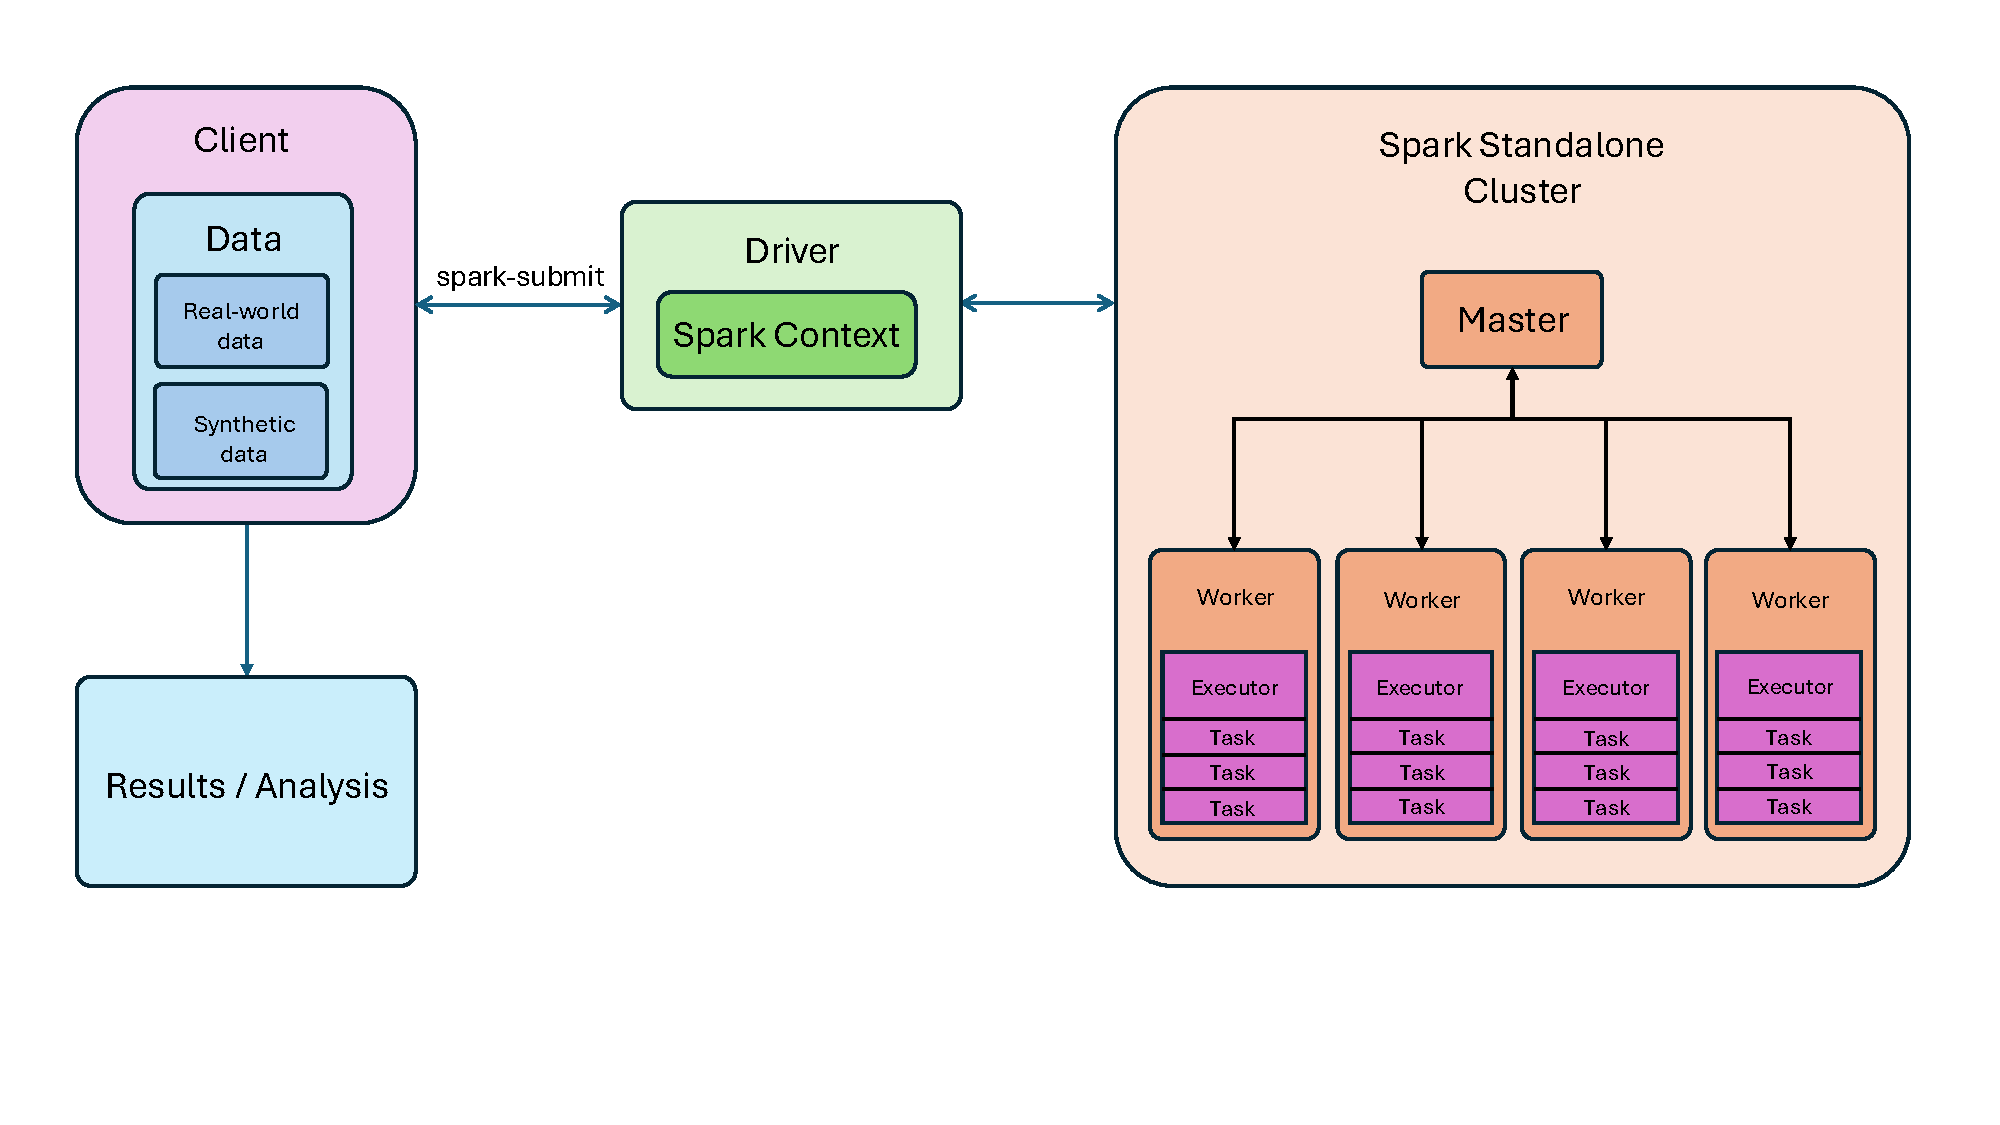
\includegraphics[width=\linewidth]{images/Workflow_image.pdf}
%     \caption{Experimental Workflow}
%     \label{fig:workflow}
% \end{figure}
Finally, the given approach combines an approximate Monte Carlo implementation with a distributed Spark environment and a systematic experimental framework. The main goal of this setup was to determine whether the described method can operate with much less memory than the standard PageRank implementation. While a trade-off in accuracy and performance was expected and tolerated, the method aims to provide sufficient accuracy and performance. The evaluation will reveal whether the Monte Carlo approach is a viable alternative to the standard PageRank method in environments with restricted memory and large-scale graphs, addressing the central research question of this thesis.


\subsection{Error Handling}
% \subsubsection{Out-of-Memory Handling}
% \subsubsection{Crash Scenarios Encountered During Experiments}
% \subsubsection{Timeout: How and when to cancel an Experiment}

When processing large-scale graphs, memory exhaustion and application crashes are inevitable. Therefore, error-handling strategies were necessary to ensure that experiments remain reproducible and manageable. For simplicity, this thesis only differentiates between out-of-memory (OOM) failures and timeouts. \par
The Java Out-of-Memory exception is a common scenario that was expected in this experimental setup because the goal was to deliberately strain memory. This exception is usually thrown when there is not enough memory in the Java heap to allocate to an object. This means the garbage collector is unable to free up enough space for the object. In these experiments, the exception was detected in the log files. In that case, the configurations were automatically marked as failed and excluded from further experiments. \par
Since very large graphs were being processed, some experiments can take a disproportionately long time to finish. This is why a timeout mechanism was implemented to prevent experiments from blocking the pipeline. If an experiment did not finish within the predefined time, the current experiment was terminated, and the next experiment with different configurations started. This ensures that all experiments finished within an acceptable time frame.  \par
These error handling strategies established a more systematic and stable process. Experiments could run without manual intervention, and the resulting datasets are more consistent.

% \subsection{Datasets}
 


% \subsubsection{Data Sources of real-world Graphs}
% % Description of synthetic and real-world datasets used.

\subsection{Allocated Memory}
The main goal of this thesis was to investigate wether the Monte Carlo PageRank approach is able to operate on restrained memory and compare it to the standard PageRank approach. Therefore, allocated memory was analyzed as the key evaluation metric. 
\vspace{0.5em}
\begin{lstlisting}[language=bash, caption={Spark-submit command}]
spark-submit \
  --class "$SPARK_APP_CLASS" \
  --master spark://casa-ubu.eecsit.tu-berlin.de:7077 \
  --name "Demo-$base-$EXECUTOR_MEM" \
  --deploy-mode client \
  --driver-memory 3g \
  --executor-cores 2 \
  --conf spark.cores.max=8 \
  --executor-memory "$EXECUTOR_MEM" \
\end{lstlisting}
\vspace{0.5em}
In Spark, the executor memory is allocated through spark-submit, which is shown above. The parameter executor-memory specifies the available JVM heap size per executor. For all experiments the allocated memory per executor was varied and set between 450 MiB and 8 GiB. Other parameters such as the number of executors and total numbers of cores were kept the same to ensure comparability throughout all experiments.\par
The memory configurations were logged for both the Monte Carlo method and the standard method. In case the allocated memory was not sufficient for the application and an OOM exception was thrown, the error was handled as mention above. The failed runs show the boundaries of each method under limited memory. The focus of the analysis is put on the minimum memory required and how this changes with increasing the graph size. The results are comapred between the two methods.



\subsection{Runtime}
Runtime is another metric that was analyzed in this thesis. It shows how both methods perform under limited memory conditions. Although a trade-off in runtime was considered as acceptable, the methods should aim to finish within an acceptable time under the given circumstances. It also shows the practicality of both methods.\par
Therefore, a timeout of 30 minutes was implemented and the experiments were handled according to the error handling section.\par 
The total runtime of each experiment was measured from when the Spark application was submitted until the Spark Session was stopped. The shell scripts that automated the experiments also logged the runtime and the configurations, which ensures an identical setup across all experiments.\par
The analyses focuses mainly on the effect of different graph sizes on the runtime. 


\subsection{Accuracy}
The accuracy was evaluated by comparing the ranks of the Monte Carlo method and the standard PageRank method. The standard PageRank method is considered to be the ground truth as it was configured with a tolerance of $0.001$. During the experiments the goal was to determine how close ranks are to the ground truth. Accuracy is mainly controlled by the number of walkers, the steps per walker and the graph structure. \par

Since in many real-world applications only the top ranks are needed, the goal was to only analyze the top $20$ ranks. The ranks were also collected through the shell scripts. The accuracy was then determined by the Jaccard index, which is a statistic used to measure the similarity and distance of sample sets. Jaccard index in combination with the top $20$ ranks is very simple and focuses on overlap of important nodes instead of overemphasizing tail nodes.

\vspace{1.0em}
\begin{algorithm}[H]
\caption{Jaccard Similarity}
\KwIn{Two rank lists $L_{MC}$, $L_{GX}$}
\KwOut{Similarity $s$, Distance $d$}

$S_{MC} \gets$ set($L_{MC}$) \;
$S_{GX} \gets$ set($L_{GX}$) \;

$I \gets |S_{MC} \cap S_{GX}|$ \;  
$U \gets |S_{MC}| + |S_{GX}| - I$ \; 

$s \gets I / U$ \;
$d \gets 1 - s$ \;

\Return $(s, d)$ \;
\end{algorithm}
\vspace{1.0em}

The resulting value is a percentage that represents the similarity to the ground truth. \par

The accuracy was analyzed on different graph sizes and structures. Additionally the number of walkers and the number of steps was varied across experiments. With an increasing number of walkers and steps a higher accuracy was expected. Furthermore larger and more complex graphs would require more walkers to achieve good accuracy. Also, a variance in the ranks of the Monte Carlo approach was expected since it follows the random surfer model and identical ranks are unlikely. Therefore, the average similarity of the top $20$ ranks across five different runs with the same configurations was taken to get a more representative result.


\subsection{Costs (GiB-hours)}
% Memory usage, runtime, accuracy (e.g., compared to GraphX).
A cost metric was introduced to reflect both runtime and minimal allocated memory. GiB-hours combines these two metrics to show how much cluster memory was allocated and for how long. It is the area under the memory time curve. For each experiment, it was computed by multiplying the allocated executor memory (GiB) by the runtime (hours). \par
Since the setup was constant across all experiments, the cost metric was primarily influenced by executor memory and runtime. The driver memory was also kept constant to maintain focus on executor memory during the experiments and to make to GiB-hours directly comparable across Monte Carlo and GraphX experiments. Additionally, no off-heap or reserved memory was added. Thus, the cost metric depends solely on the configured on-heap executor memory. However, GiB-hours doesn't capture all costs such as the network costs.\par
If only the runtime had been taken into account, the experiments with high memory demand would have appeared to be more favorable, even though they consumed much more memory. This is why the cost metric is crucial for providing a balanced overview. It captures both runtime and memory usage during the experiment. \par
The analysis predicted that the Monte Carlo approach would require fewer GiB-hours, while the standard PageRank method was expected to be significantly more costly.


\subsection{Results and Plots}

\begin{figure}[H]
    \centering
    \begin{subfigure}[t]{0.73\linewidth}
        \centering
        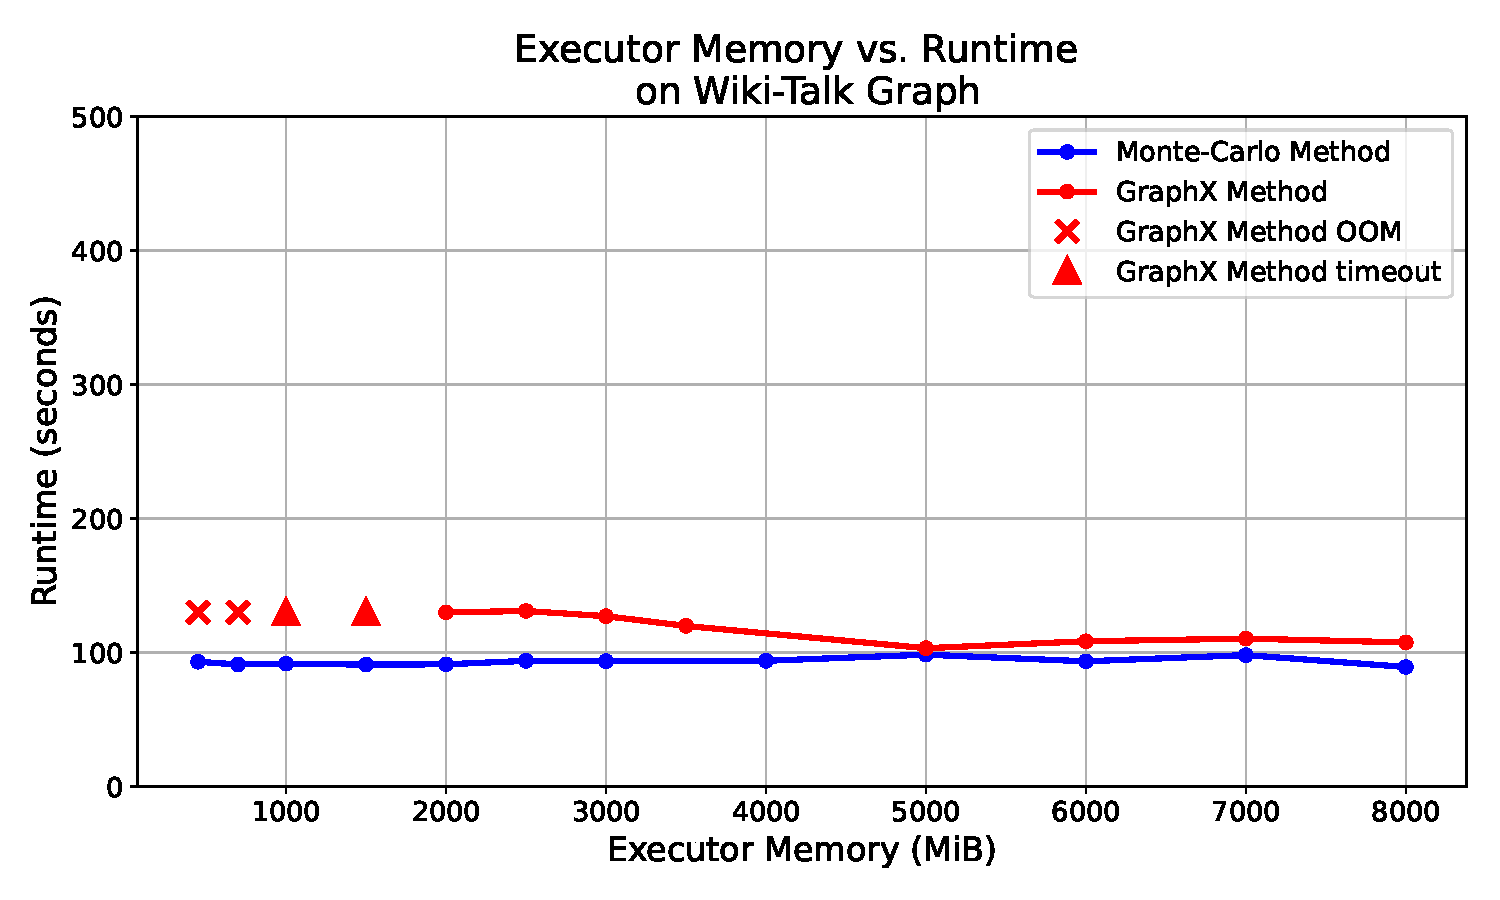
\includegraphics[width=\linewidth]{images/plots/wiki-Talk/memory_vs_runtime_3wpn_v2.pdf}
        \caption{Memory vs. Runtime}
        \label{fig:wikirun}
    \end{subfigure}\hfill
    \begin{subfigure}[t]{0.73\linewidth}
        \centering
        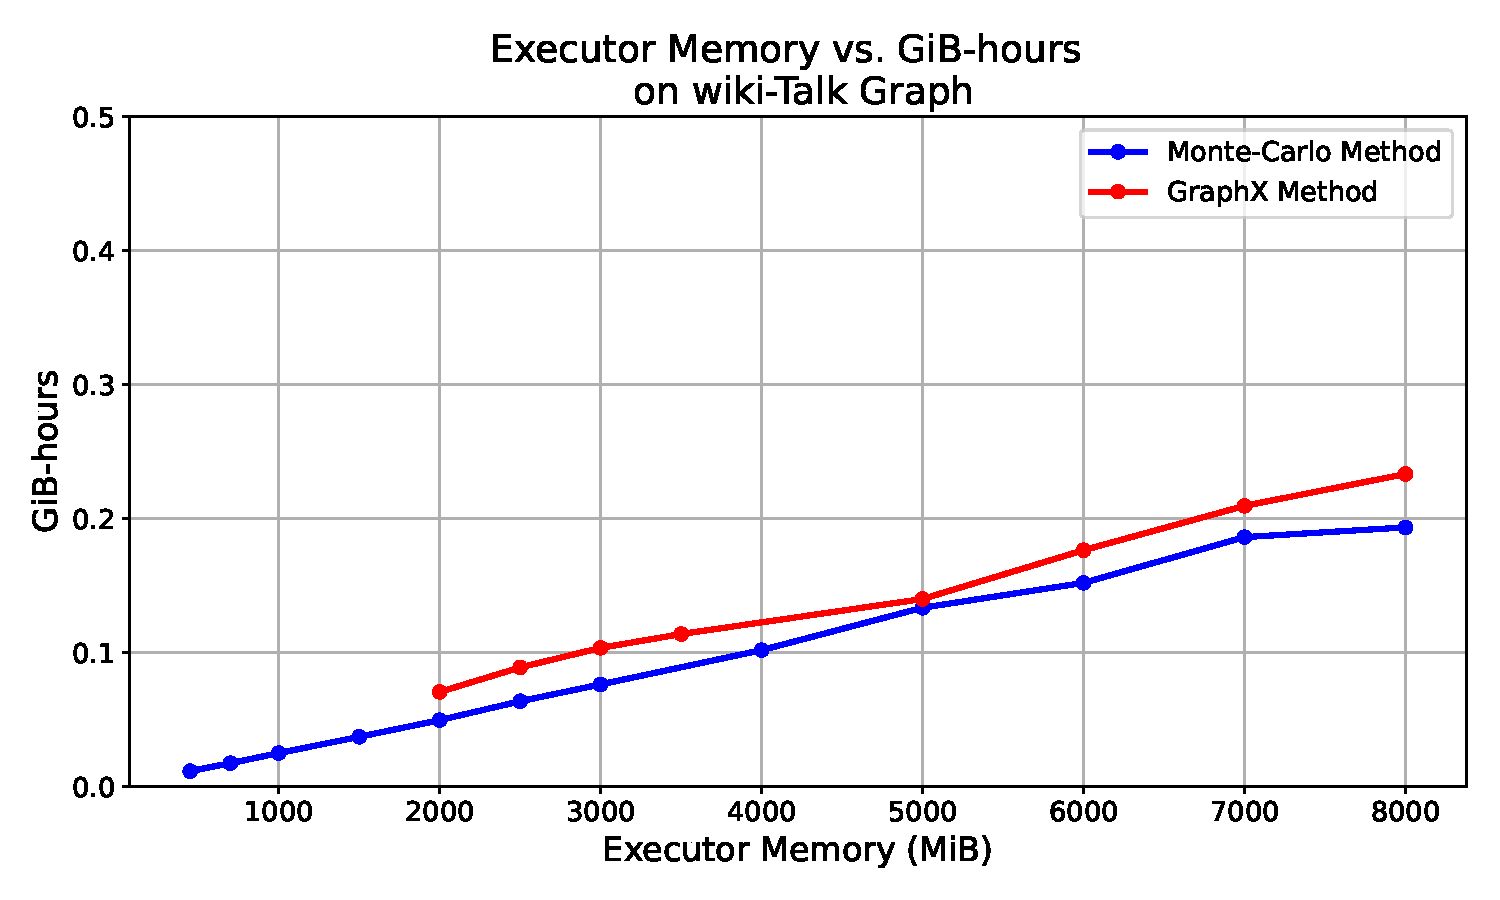
\includegraphics[width=\linewidth]{images/plots/wiki-Talk/gbhrs_nodes_v2.pdf}
        \caption{GiB-hours}
        \label{fig:wikigibhrs}
    \end{subfigure}
    % \begin{subfigure}[t]{0.48\linewidth}
    %     \centering
    %     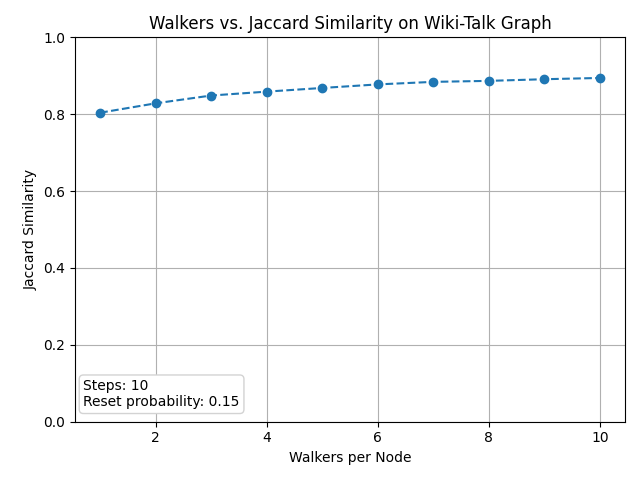
\includegraphics[width=\linewidth]{images/plots/wiki-Talk/steps_vs_accuracy_server_edited.png}
    %     \caption{GiB-hours}
    %     \label{fig:wikiacc}
    % \end{subfigure}
    \caption{Comparison with 3 walkers per node, 10 steps per walker}
    \label{fig:wiki-comparison}
\end{figure}

% \begin{figure}[H]
%     \centering
%     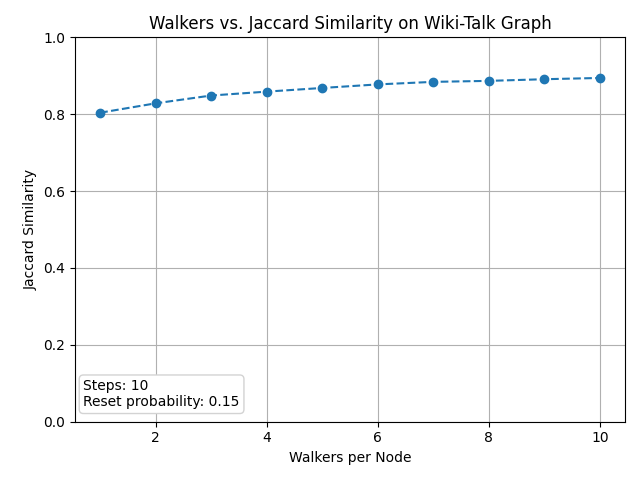
\includegraphics[width=\linewidth]{images/plots/wiki-Talk/steps_vs_accuracy_server_edited.png}
%     \caption{Accuracy}
%     \label{fig:wikiacc}
% \end{figure}

\begin{figure}[H]
    \centering
    \begin{subfigure}[t]{0.47\linewidth}
        \centering
        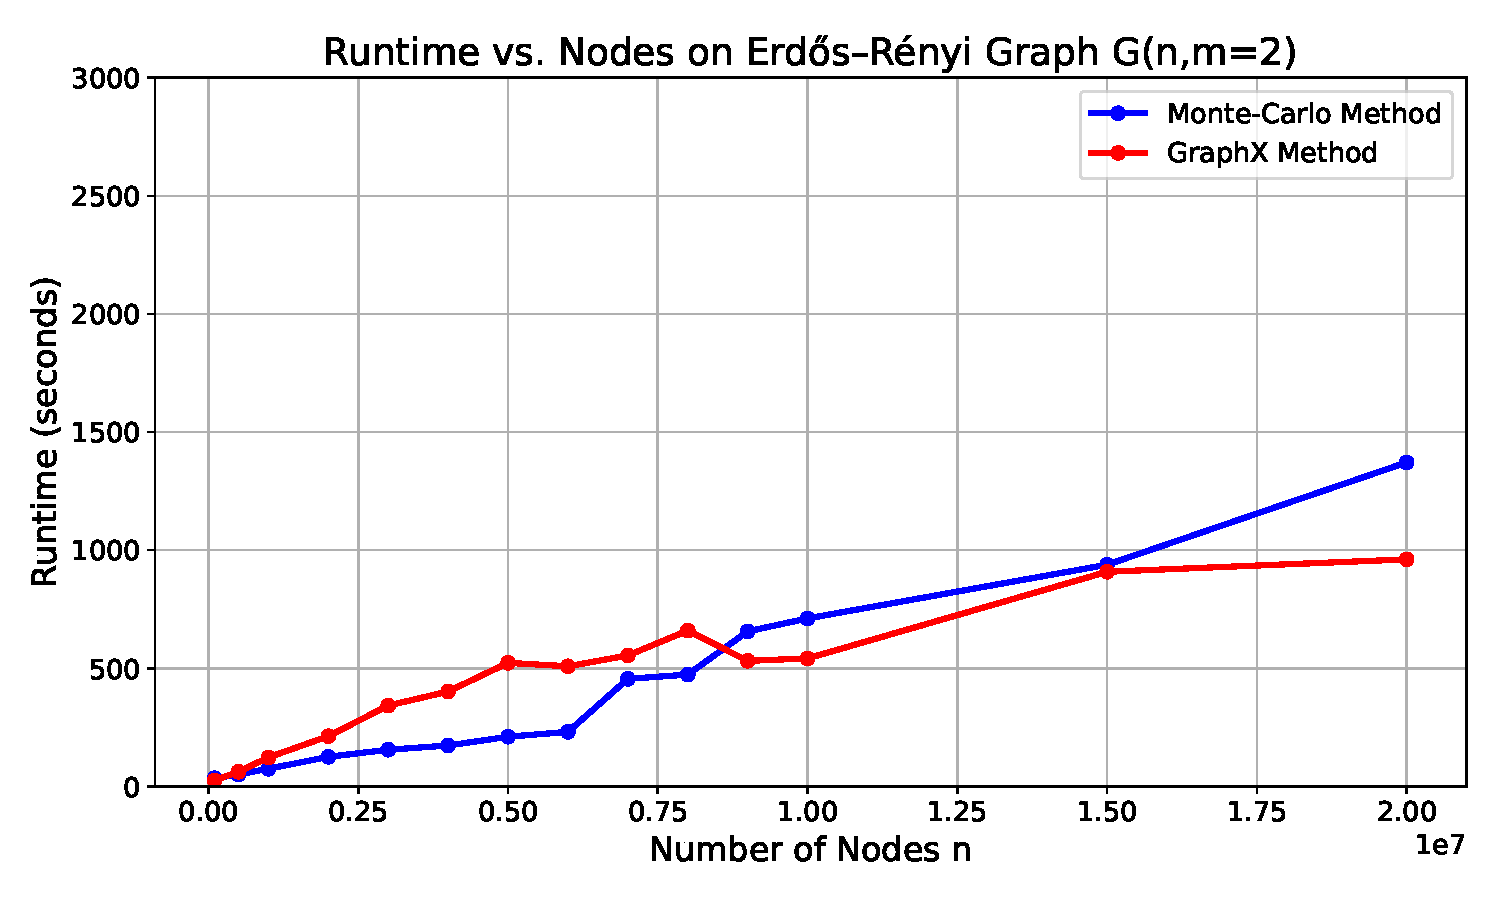
\includegraphics[width=\linewidth]{images/plots/ER_2edg/runtime_vs_nodes_er_graph_2_edges.pdf}
        \caption{2 edges per node}
        \label{fig:2run}
    \end{subfigure}\hfill
    \begin{subfigure}[t]{0.47\linewidth}
        \centering
        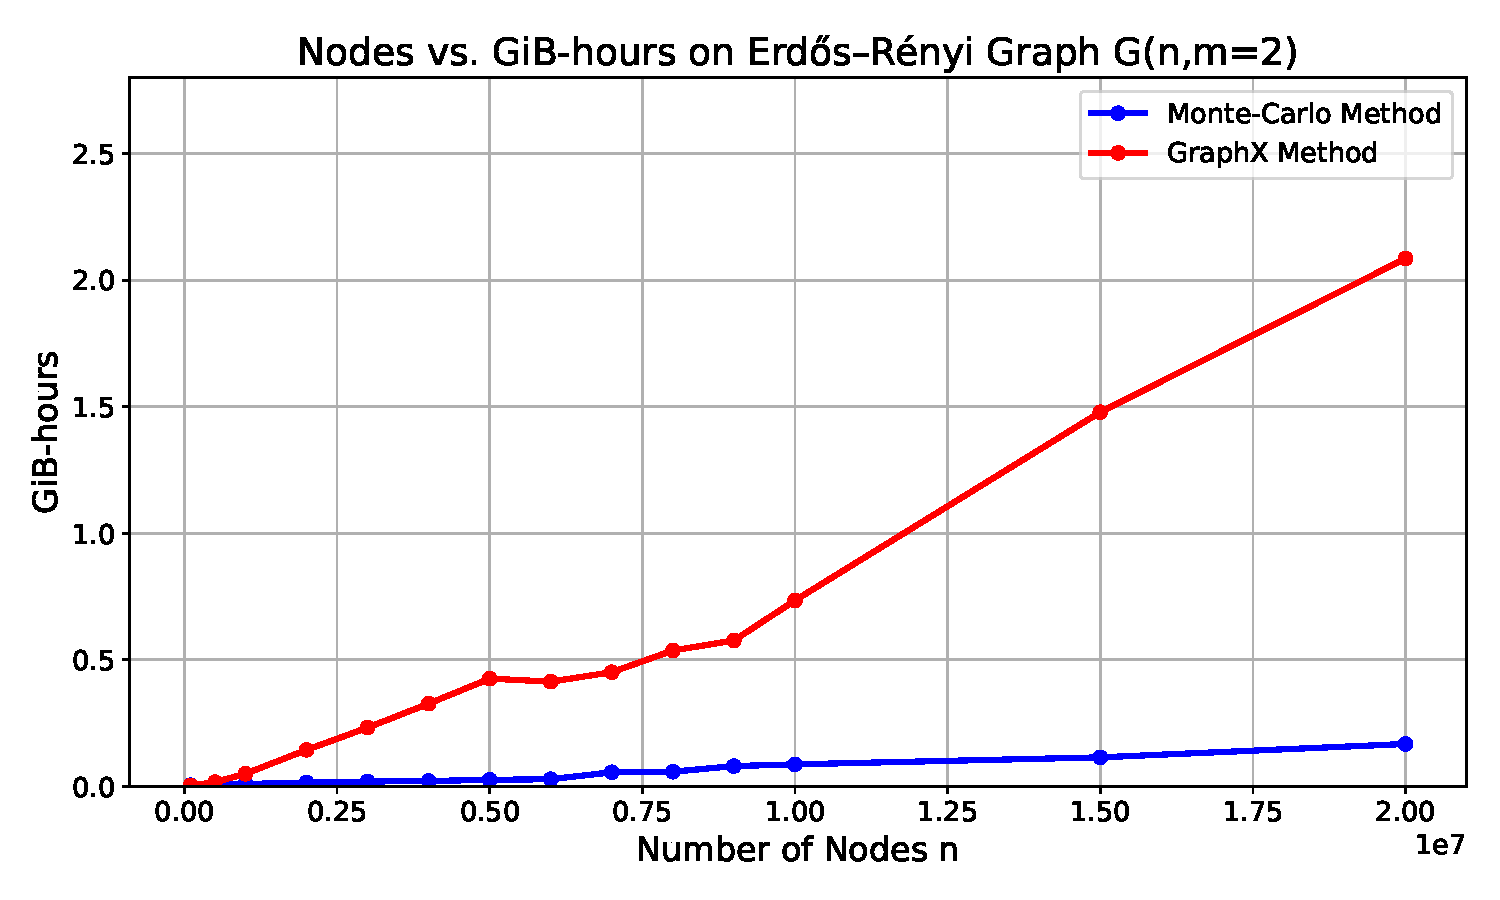
\includegraphics[width=\linewidth]{images/plots/ER_2edg/gbhrs_nodes_er_graph_2edges.pdf}
        \caption{2 edges per node}
        \label{fig:2cost}
    \end{subfigure}
    \begin{subfigure}[t]{0.47\linewidth}
        \centering
        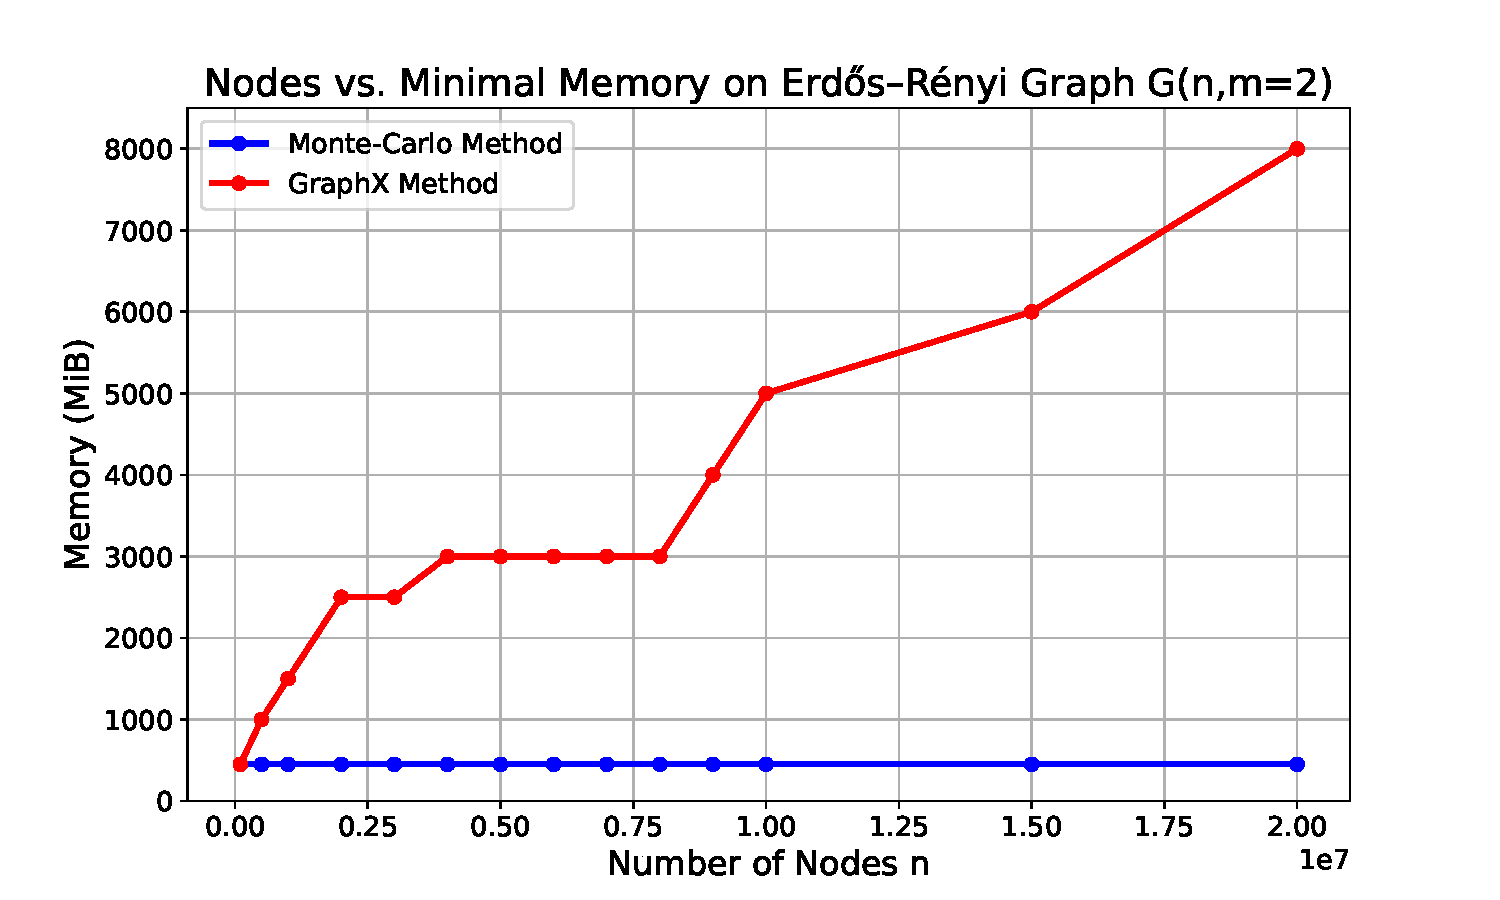
\includegraphics[width=\linewidth]{images/plots/ER_2edg/nodes_vs_mvm_2edges.pdf}
        \caption{2 edges per node}
        \label{fig:2mvm}
    \end{subfigure}\hfill
\end{figure}

\begin{figure}[H]
    \centering
    \begin{subfigure}[t]{0.47\linewidth}
        \centering
        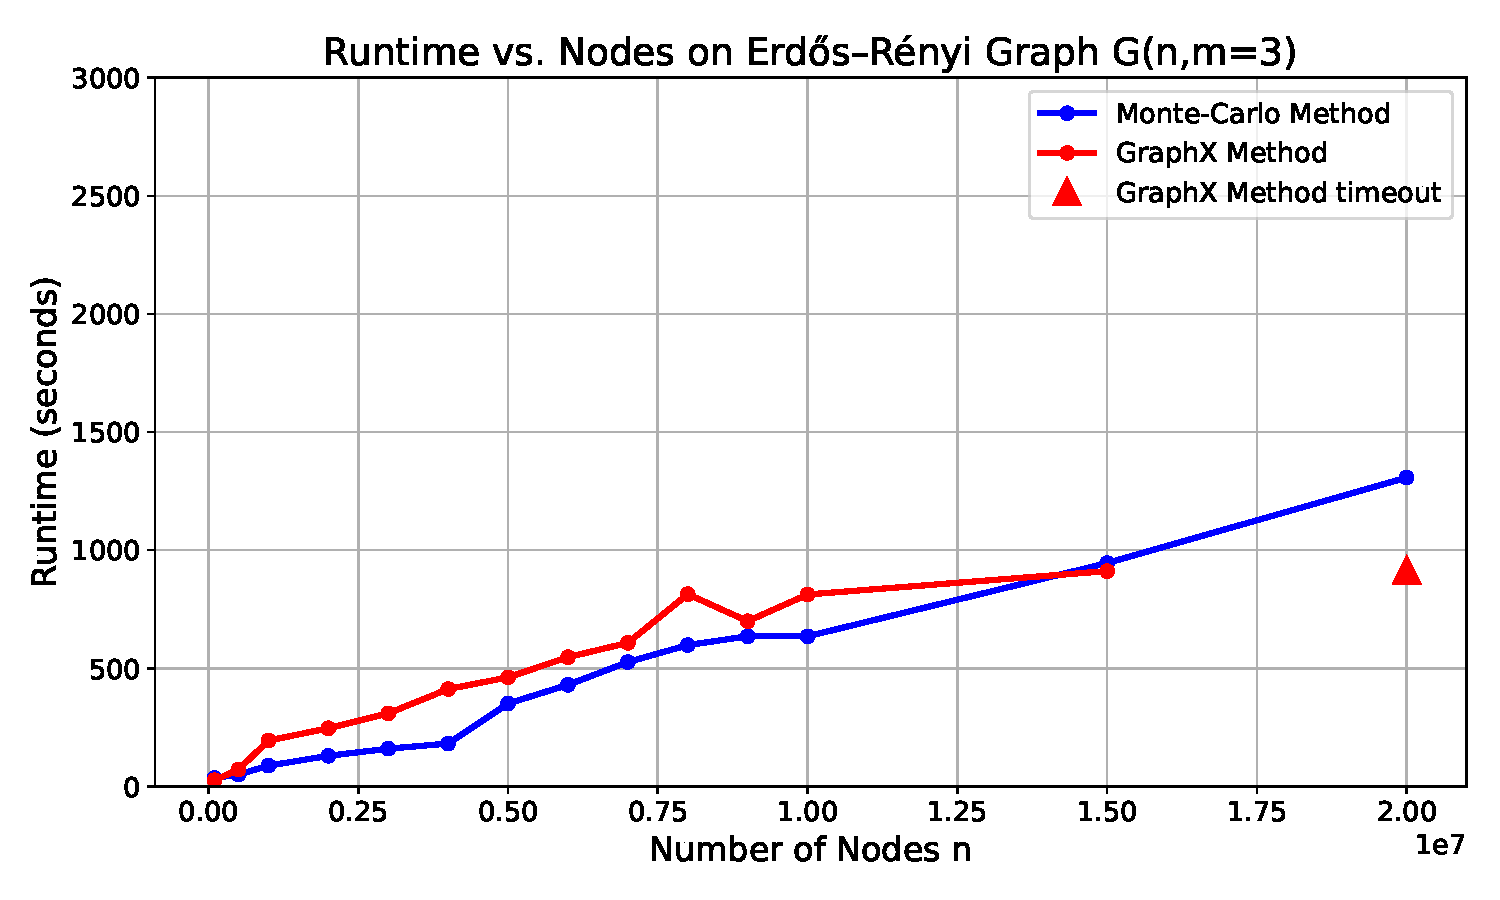
\includegraphics[width=\linewidth]{images/plots/ER_3edg/runtime_vs_nodes_er_graph_3_edges.pdf}
        \caption{3 edges per node}
        \label{fig:3run}
    \end{subfigure}
    \begin{subfigure}[t]{0.47\linewidth}
        \centering
        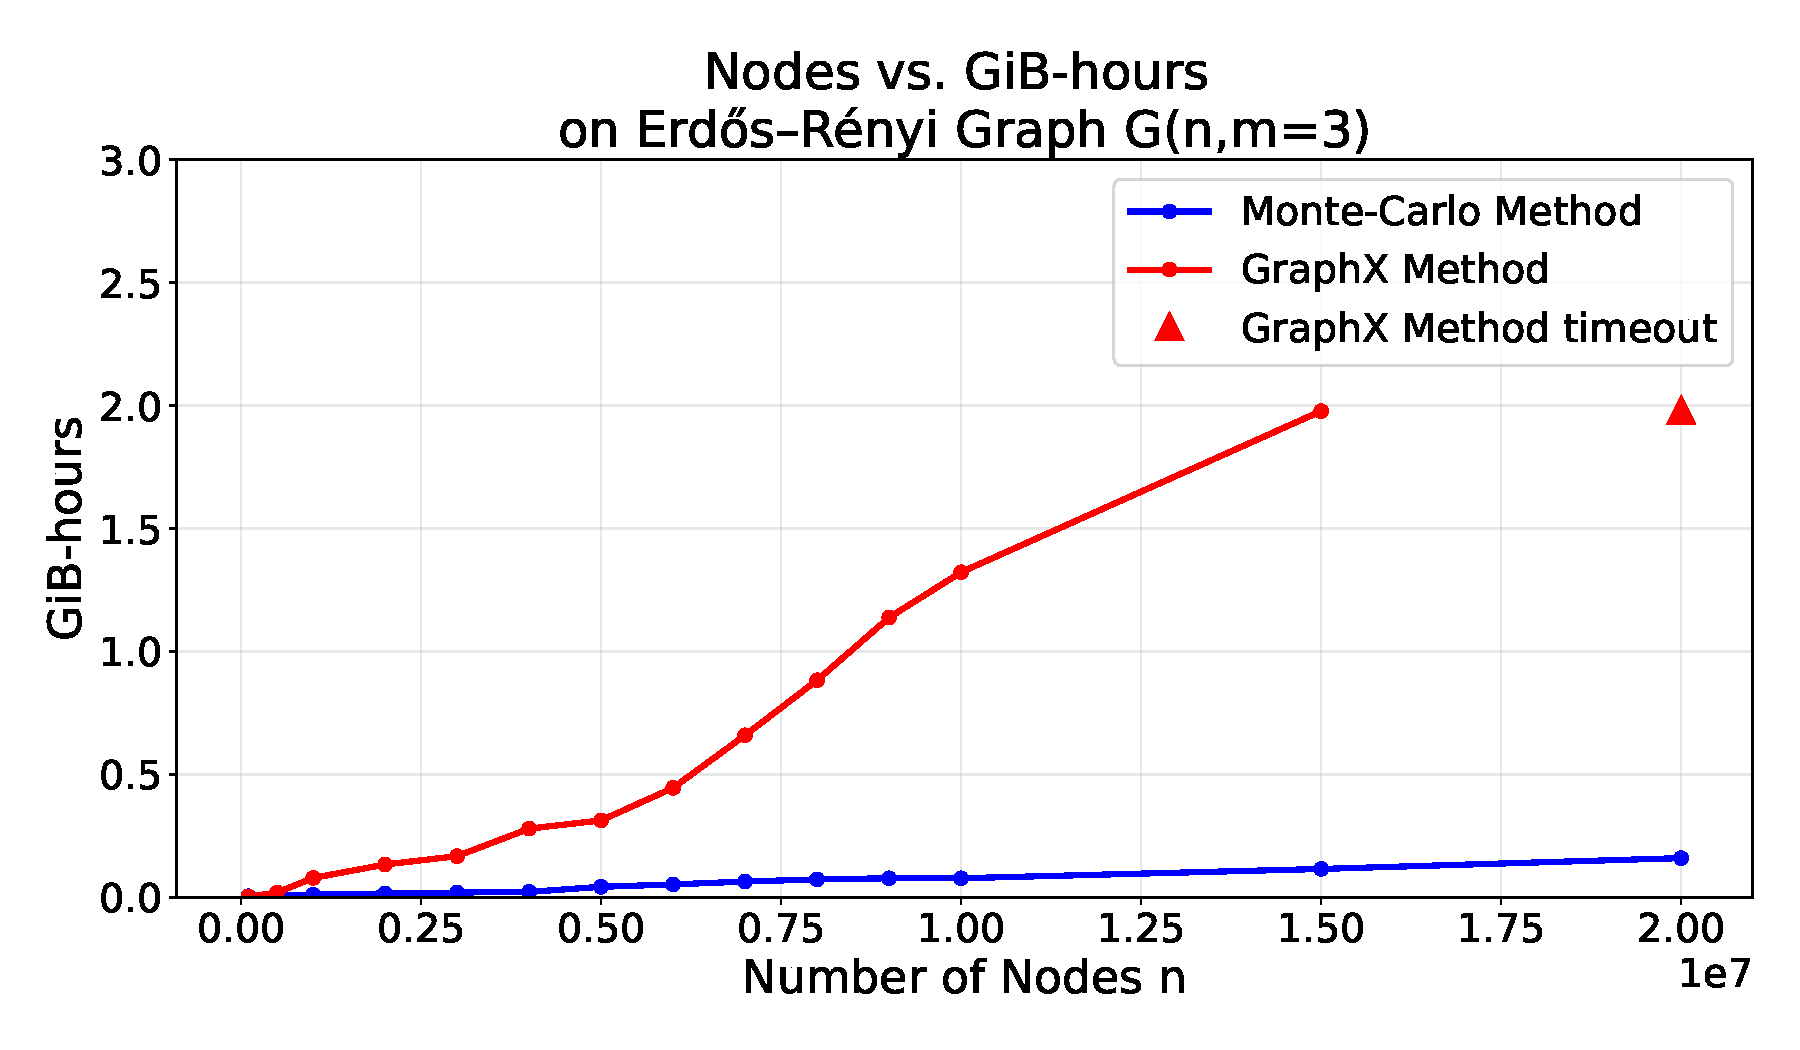
\includegraphics[width=\linewidth]{images/plots/ER_3edg/gbhrs_nodes_er_graph_3edges.pdf}
        \caption{3 edges per node}
        \label{fig:3cost}
    \end{subfigure}
    \begin{subfigure}[t]{0.47\linewidth}
        \centering
        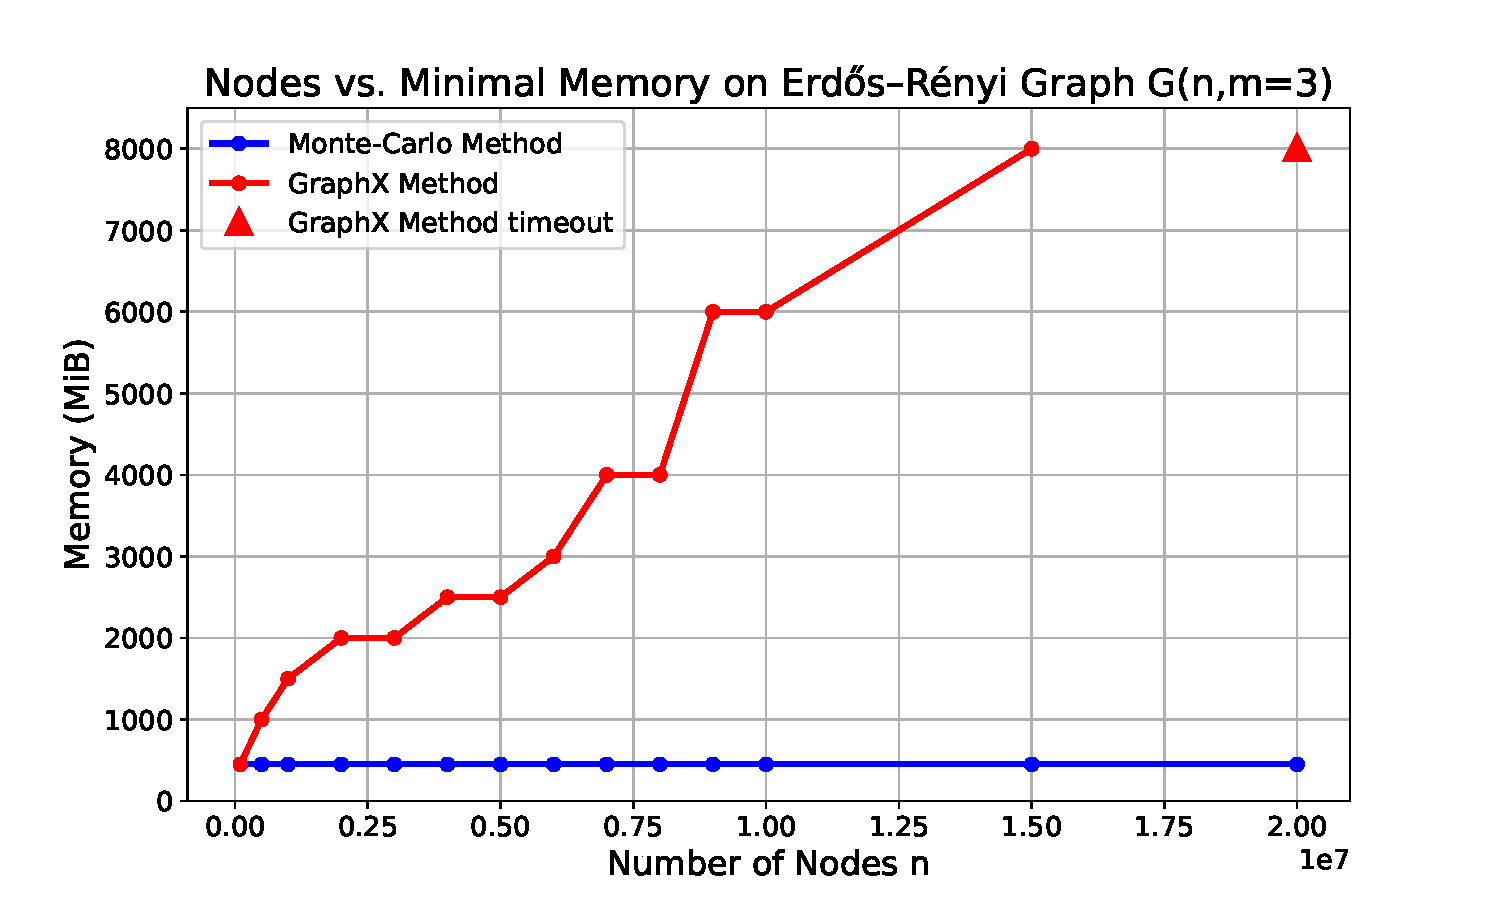
\includegraphics[width=\linewidth]{images/plots/ER_3edg/nodes_vs_mvm_3edges.pdf}
        \caption{3 edges per node}
        \label{fig:3mvm}
    \end{subfigure}
\end{figure}

\begin{figure}[H]
    \centering
    \begin{subfigure}[t]{0.47\linewidth}
        \centering
        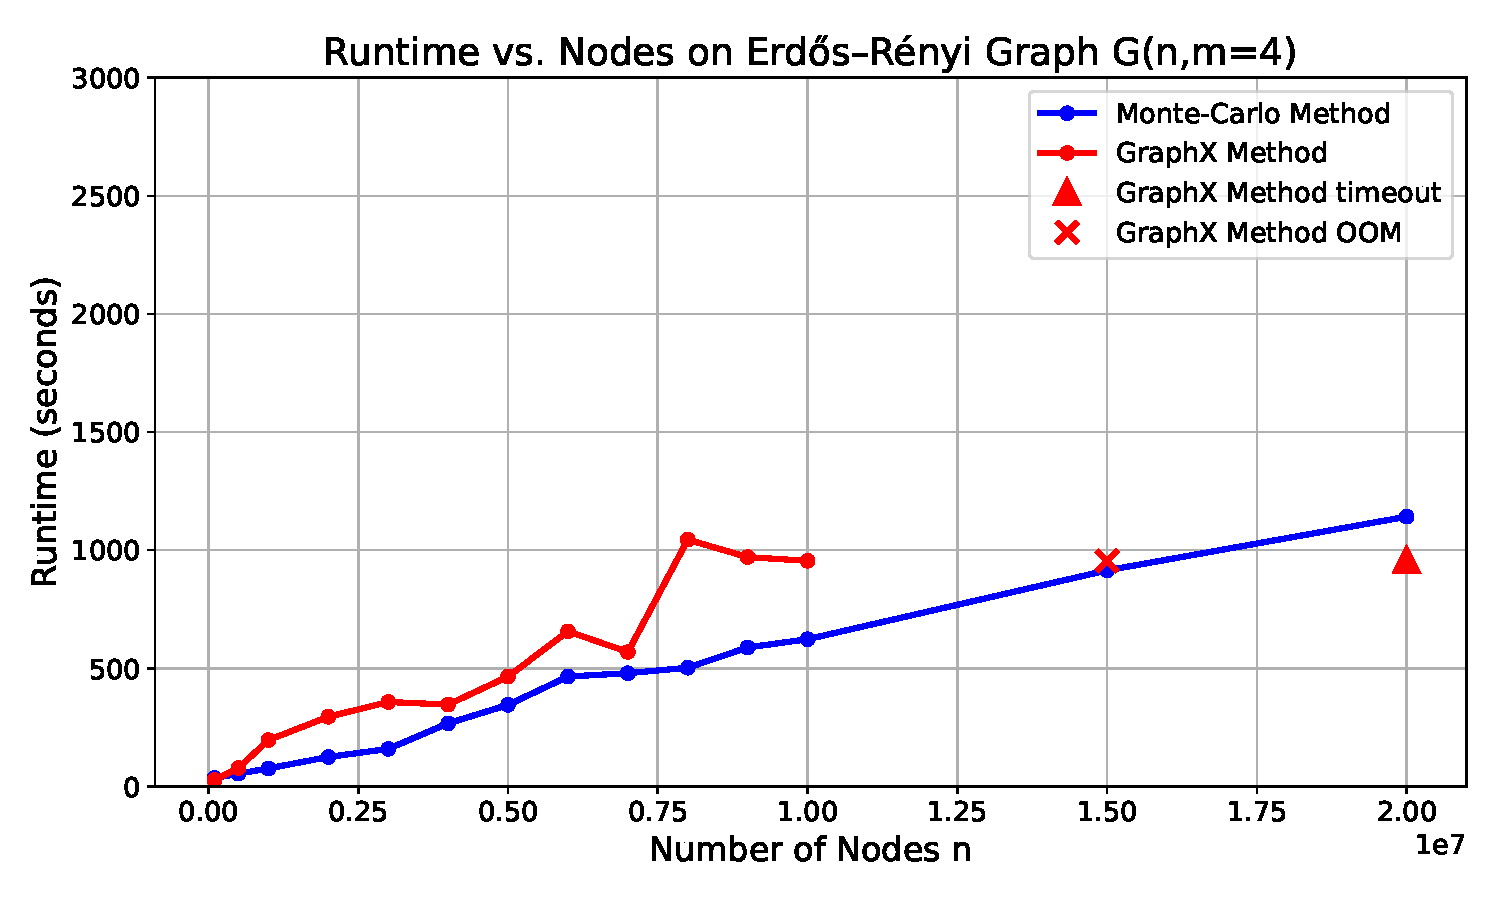
\includegraphics[width=\linewidth]{images/plots/ER_4edg/runtime_vs_nodes_er_graph_4_edges.pdf}
        \caption{4 edges per node}
        \label{fig:4run}
    \end{subfigure}
    \begin{subfigure}[t]{0.47\linewidth}
        \centering
        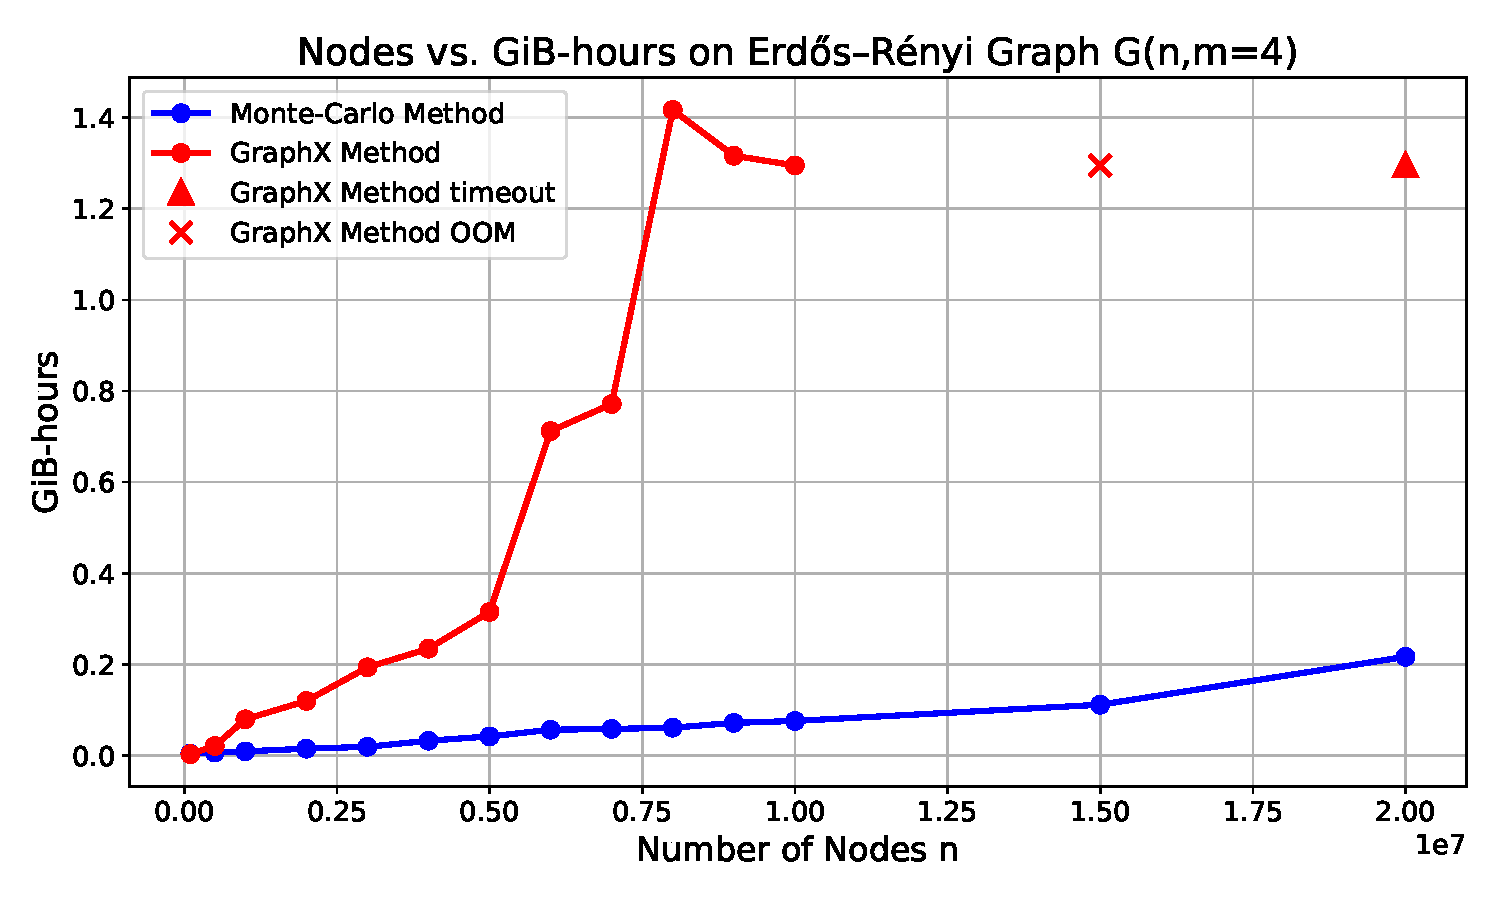
\includegraphics[width=\linewidth]{images/plots/ER_4edg/gbhrs_nodes_er_graph_4edges.pdf}
        \caption{4 edges per node}
        \label{fig:4cost}
    \end{subfigure}
    \caption{3 walkers per node and 10 steps per walker}
\end{figure}

\begin{figure}[H]
    \centering
    \begin{subfigure}[t]{0.47\linewidth}
        \centering
        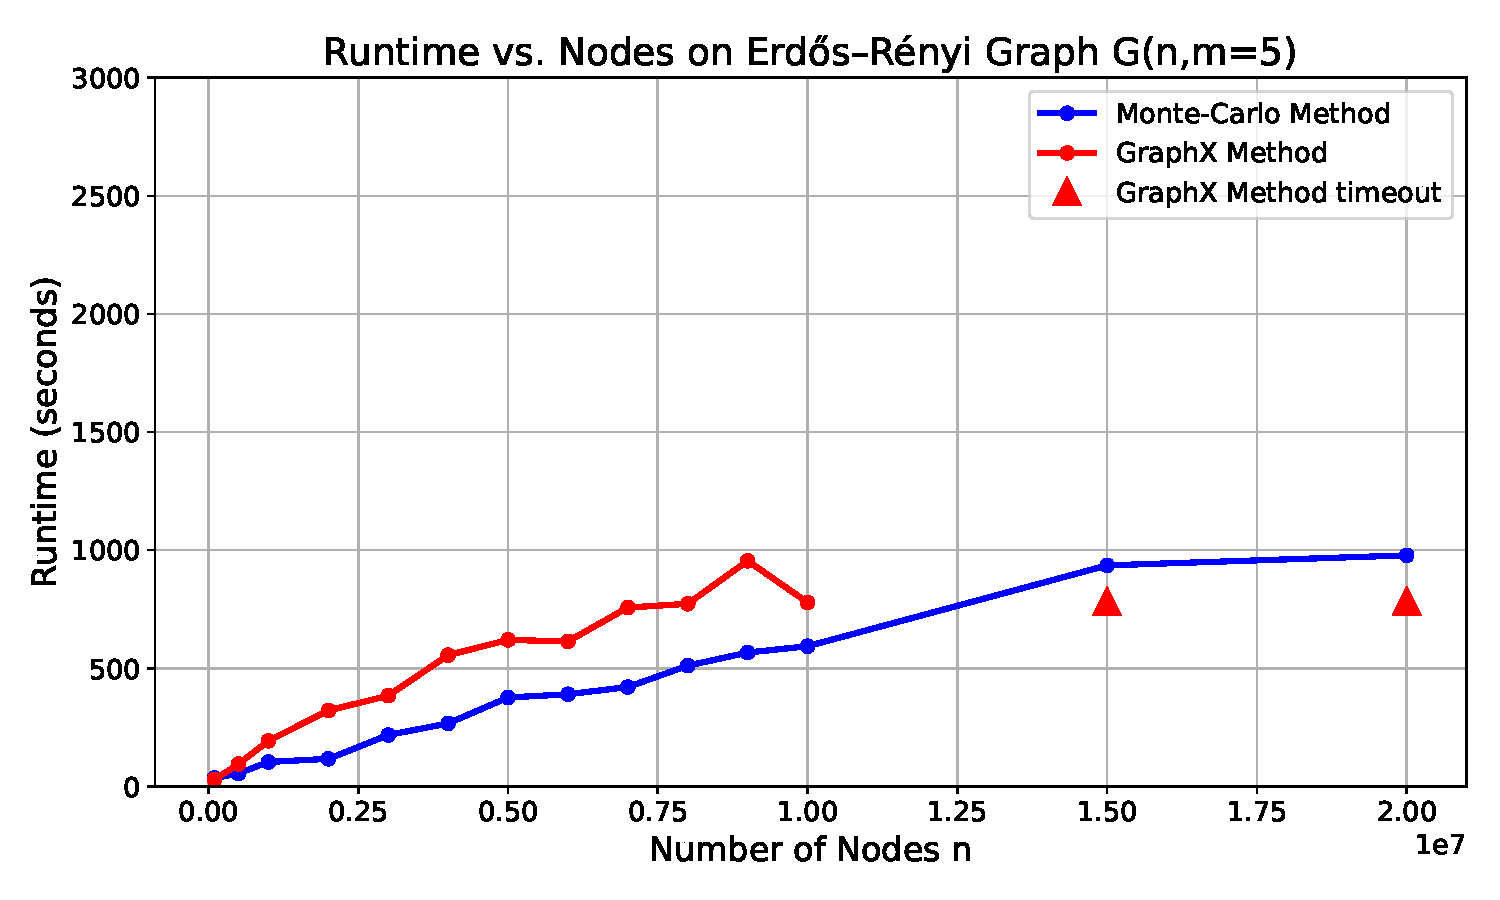
\includegraphics[width=\linewidth]{images/plots/ER_5edg/runtime_vs_nodes_er_graph_5_edges.pdf}
        \caption{5 edges per node}
        \label{fig:5run}
    \end{subfigure}
    \begin{subfigure}[t]{0.47\linewidth}
        \centering
        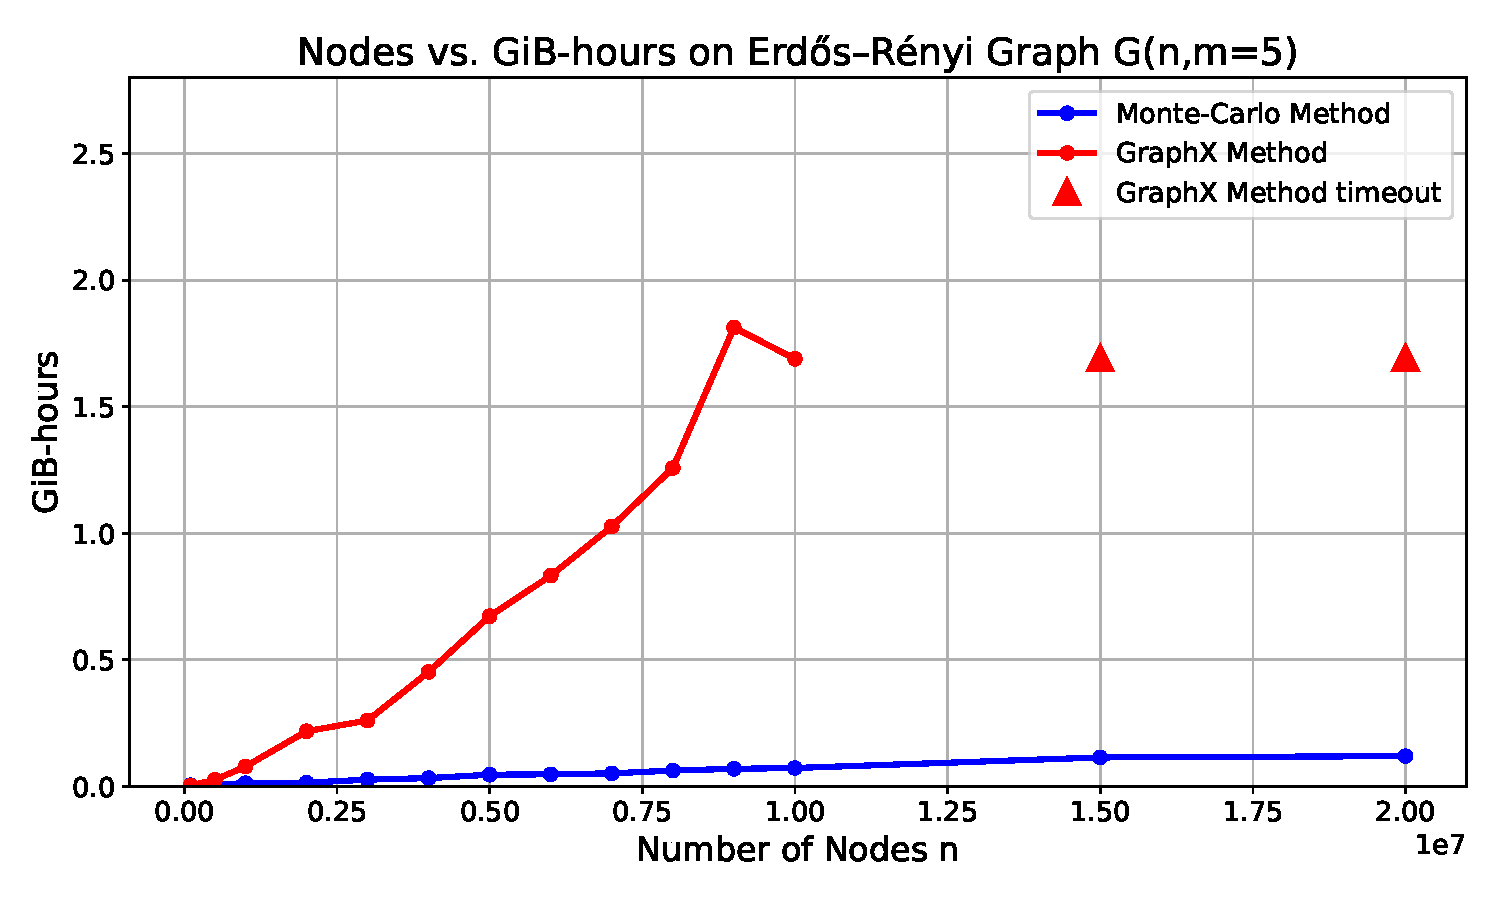
\includegraphics[width=\linewidth]{images/plots/ER_5edg/gbhrs_nodes_er_graph_5edges.pdf}
        \caption{5 edges per node}
        \label{fig:5cost}
    \end{subfigure}
    \begin{subfigure}[t]{0.47\linewidth}
        \centering
        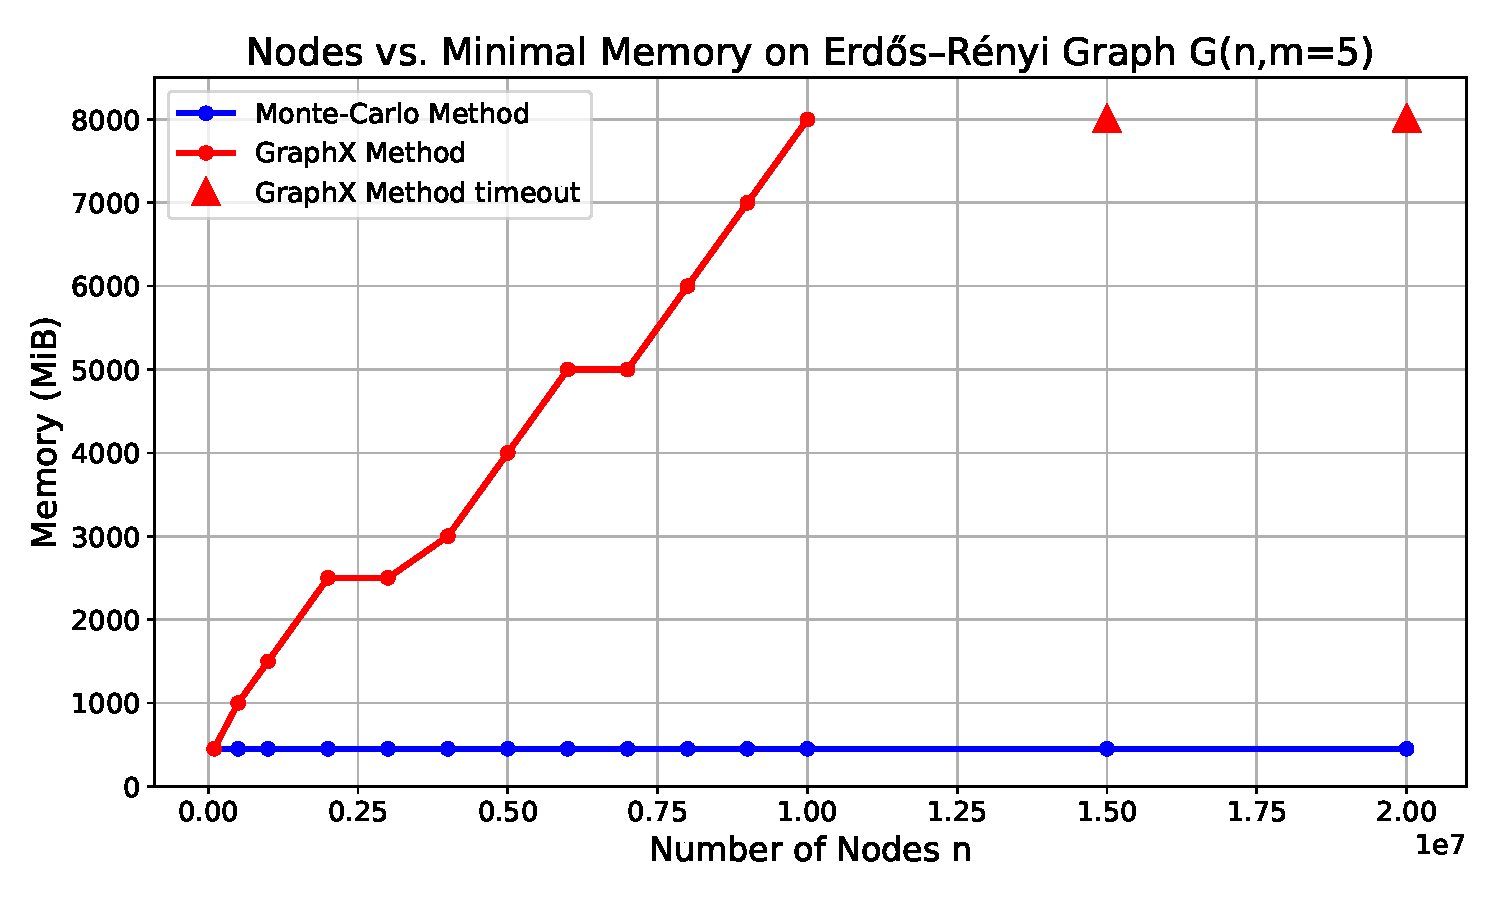
\includegraphics[width=\linewidth]{images/plots/ER_5edg/nodes_vs_mvm_5edges.pdf}
        \caption{5 edges per node}
        \label{fig:5mvm}
    \end{subfigure}
\end{figure}

%%%%%%% ER Graphs %%%%%%%
Next the plots of the synthetic graphs are analyzed. 


\subsubsection{Performance Plots}
\subsubsection{Accuracy Plots}
\subsubsection{Cost Plots}
\subsubsection{Graph Size vs. Runtime/Memory Plots}
% Include figures/tables: performance vs. accuracy vs. memory.

\subsection{Discussion}
\subsubsection{Trade-offs}
\subsubsection{Experimental setup: realistic?}
\subsubsection{Monte Carlo Approach: good Alternative?}
% Interpret results and explain when your approach is advantageous.
